


% \begin{table}[]
\centering
        \caption{Filtering Results}
        \label{tab:filter}
        \resizebox{0.45\textwidth}{!}{%
            \begin{tabular}{|l|r|r|r|}
            \hline
            \thead{Cases} & \thead{\#Critical Edges} & \thead{Missing Point} & \thead{\#Non-critical Edges at Missing Point}\\\hline
            2File                     & 3                        & 9.49          & 0                                     \\\hline
            3File                     & 4                        & 6.49          & 0                                     \\\hline
            Python-wget               & 4                        & 5.19          & 1                                     \\\hline
            Python-wget-unzip         & 8                        & $<0.01$          & 60                                    \\\hline
            Shell-script              & 4                        & 3.15          & 1                                     \\\hline
            Shell-wget                & 4                        & 0.04          & 6                                     \\\hline
            Shell-wget-unzip          & 6                        & 2.83          & 3                                     \\\hline
            USB-merge                 & 6                        & 2.11          & 0                                     \\\hline
            curl                      & 4                        & 12.80         & 1                                     \\\hline
            scp                       & 3                        & 8.29          & 4                                     \\\hline
            wget                      & 2                        & 6.20          & 29                                    \\\hline
            command-injection-c1 & 2                        & 17.00         & 49                                    \\\hline
            command-injection-c2 & 3                        & 286.50        & 0                                     \\\hline
            data-leakage             & 5                        & 302.89        & 0                                     \\\hline
            password-crack-c1    & 2                        & 9.00          & 34                                    \\\hline
            password-crack-c2    & 4                        & 14.20         & 1                                     \\\hline
            password-crack-c3    & 4                        & $<0.01$          & 57                                    \\\hline
            penetration-c1         & 3                        & 0.02          & 5                                     \\\hline
            penetration-c2         & 11                       & $<0.01$          & 21                                    \\\hline
            vpnfilter-c1          & 2                        & 4.67          & 12                                    \\\hline
            vpnfilter-c2          & 3                        & 3.60          & 15                                   \\\hline 
            \thead{average}    & 4                        & 32.92          &14.24 \\\hline
            \end{tabular}
        }
\end{table}
% \begin{figure}[!ht]
%     \centering
%     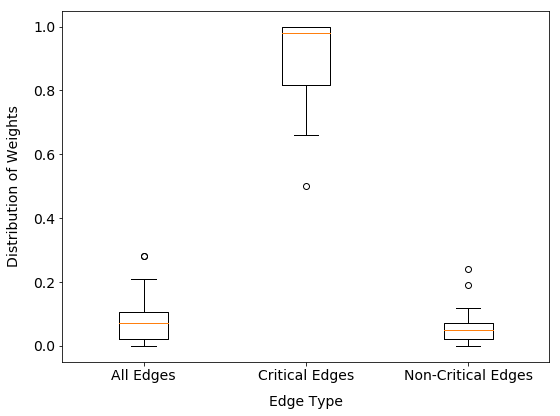
\includegraphics[width=0.48\textwidth]{figs/weight-box-avg.png}
%     \caption{Box plot showing the difference in weights between critical edges and non-critical edges.}
%     %\dcaption{All missing points distribute between $T = 0.25$ and $T = 1.0$.}
%     \label{fig:box}
% \end{figure}



\subsubsection{Revealing Critical Edges Based on Edge Weights}
\label{subsec:graphreduction}

% \begin{figure}[!ht]
%     \centering
%     \includegraphics[width=0.48\textwidth]{figs/fig:edge-thresh.pdf}
%     \caption{Effectiveness of filtering. The percentage of edges remaining after filtering drops significantly at $T = 0.10$ and remains stable below 10\%.}
%     %\dcaption{The percentage of edges remaining after filtering drops significantly at $T = 0.10$ and remains stable below 10\%.}
%     \label{fig:edge-thresh}
% \end{figure}


% \begin{figure}[!ht]
%     \centering
%     \includegraphics[width=0.48\textwidth]{figs/fig:cdf.pdf}
%     \caption{Critical edge loss from filtering. All missing points are distributed between $T = 0.25$ and $T = 1.0$.}
%     %\dcaption{All missing points distribute between $T = 0.25$ and $T = 1.0$.}
%     \label{fig:cdf}
% \end{figure}




\cref{tab:summary} shows the detailed summary of statistics of using \tool to investigate all the $18$ attack cases. 
As we can see, the number of nodes and the number of edges in the dependency graph are 412 and 19,394 on average, and can be as large as 4,252 and 151,200, while the number of critical edges are generally quite small ($<=5$), which is consistent with previous studies~\cite{mcitracking,ma2016protracer,backtracking,backtracking2}.
Thus, it is non-trivial to reveal these edges from the massive non-critical edges.

\myparatight{Edge Weight Distribution}
\cref{fig:box} shows the distribution of average weight of critical edges and non-critical edges in each case using a box plot.
We can see that the average weights of critical edges are significantly higher than that of non-critical edges. 
Note that the average weight of all edges are close to the average weight of non-critical edges because most of the edges are non-critical. 

\myparatight{Filtering Non-Critical Edges}
% The important goal of \sys is to filter out as many irrelevant edges as possible while preserving critical edges in the dependency graph.
\tool hides non-critical edges whose weights are below a threshold.
To provide a guidance on choosing this threshold, we test the filtering performance on all attack cases
%attacks studied 
in \cref{subsec:cases}
by selecting a range of values from 0.05 to 0.95 with a pace of 0.05 as 
%the 
thresholds. 
% The edges whose weights are below this number are hidden.
\cref{fig:edge-thresh} shows the average percentage of remaining edges after edge filtering. We observe that when the threshold reaches 0.10, the average percentage of remaining edges is 9.8\%, and further increasing the threshold from 0.10 to 0.90 only results in a slightly increased amount of pruned edges (2.2\%). Such results indicate that most of the edges having reputation scores below 0.10 or above 0.90. 

While a higher threshold can hide more irrelevant edges, it may cause the loss of critical edges as well.
Thus, we define the \emph{missing point} as the greatest threshold that preserves all the critical edges for a dependency graph, 
and measure the missing points for all attack cases, as shown in \cref{fig:cdf}.
We observe that:
(1) all missing points are greater than 0.25,
and (2) about 80\% of the missing points are greater than 0.90.

Combining the results in \cref{fig:edge-thresh} and \cref{fig:cdf},
we can conclude that \emph{the weight scores of almost all the critical edges are above 0.90, while the weight scores of most of the non-critical edges are below 0.10}.
Such results clearly demonstrate the effectiveness of \tool in leveraging the discriminative weights (\cref{subsec:weight-computation}) to reveal critical edges from non-critical edges.
Furthermore, based on \cref{fig:cdf}, we can suggest an optimal range of the threshold: $\lbrack 0.1,0.25 \rbrack$.
  


\eat{
% (1) Two cases (\emph{command-injection-c2}, \emph{data-leakage}) have extremely high missing points ($T_w > 200$);
% (2) 5 out of 21 cases lost critical edges at $T_w = 2$. However, in these 5 cases, 2 of them(\emph{Shell-wget},\emph{penetration-c1}) already have less than 10 non-critical edges at missing point and 3 of them also have significant reduction in edge numbers(\cref{tab:filter}).
% (3) A plateau exists before $T_w = 2$ at a rate of 24\%. This indicate most of the cases have a missing point greater than $T_w = 2$, which proves the efficacy of our weights to differ critical edges from non-critical edges.
}

\eat{
\begin{table}[]\
\centering
    	\caption{Graph reduction results for PHASEs I and II}
    	\label{tab:Reduction}
    	\resizebox{0.48\textwidth}{!}{%
            \begin{tabular}{|l|r|r|r|r|}
            \hline
            \thead{Attacks}                & \thead{PH.I V} & \thead{PH.I E} & \thead{PH.II V} & \thead{PH.II E} \\ \hline
            3File      & 225                  & 25211             & 225            & 596         \\ \hline
            2File             & 221                  & 21100             & 221            & 537         \\ \hline
            curl                  & 212                  & 15142             & 212            & 460         \\ \hline
            shell\_script           & 229                  & 21124             & 229            & 637         \\ \hline
            python\_wget          & 162                  & 10597             & 162            & 283         \\ \hline
            scp                   & 60                   & 7912              & 60             & 78          \\ \hline
            shell\_wget           & 115                  & 4998              & 115            & 158         \\ \hline
            wget                  & 217                  & 19078             & 217            & 500         \\ \hline
            command-injection-c1      & 51                   & 65                & 51             & 51          \\ \hline
            command-injection-c2      & 1438                 & 9713              & 1438           & 2738        \\ \hline
            data-leakage       & 4252                 & 151200            & 4252           & 4261        \\ \hline
            password-crack-c1 & 35                   & 731               & 35             & 36          \\ \hline
            password-crack-c2 & 61                   & 2477              & 61             & 73          \\ \hline
            password-crack-c3 & 25                   & 58426             & 25             & 36          \\ \hline
            penetration-c1 & 60                   & 314               & 60             & 63          \\ \hline
            penetration-c2 & 30                   & 139               & 30             & 68          \\ \hline
            vpnfilter-c1      & 14                   & 274               & 14             & 14          \\ \hline
            vpnfilter-c2      & 16                   & 598               & 16             & 18          \\ \hline
            avg & 412.39 & 19394.39 & 412.39 & 589.28 \\ \hline
            \end{tabular}
        }
    % \dcaption{ .}
\end{table}

Thus, we evaluate the attack sequence reconstruction via two aspects:
(1) graph reduction and (2) revealing critical edge.

\myparatight{Graph Reduction}
\cref{tab:Reduction} shows the reduction in terms of the number of nodes (Columns ``PH.I V'' and ``PH.II V'') and in the number of edges  (Columns ``PH.I E'' and ``PH.II E'') after causality analysis in Phase I (\cref{subsec:graph-generation}) and edge merge in Phase II (\cref{subsec:graph-preprocessing}).
As we can see, the reduction is significant: the biggest graph generated by \tool only contains 4252 nodes and 4261 edges (``data-leakage'' in \cref{tab:Reduction}) considering the 24-hour log contains about \emph{2 billion} events.

\myparatight{Revealing Critical Edge}
}